\section{Esercizio 10 -- UART-RS232}
\subsection{Esercizio 10.1}
L'obiettivo è progettare un sistema di comunicazione seriale UART tra due unità, A e B, che condividono lo stesso segnale di clock. L'unità A legge dati da una memoria ROM e li invia all'unità B, che li riceve e li memorizza in una memoria MEM tramite un'interfaccia UART-RS232 [Figure \ref{fig:uart}, \ref{fig:10_UART-RS232}].

\begin{figure}[h]
    \centering
    \begin{minipage}[c]{0.45\linewidth}
        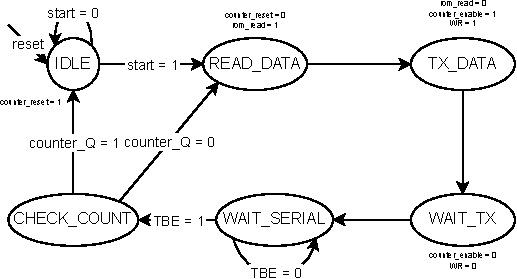
\includegraphics[width=\linewidth]{img/uart_A.pdf}
    \end{minipage}
    \hfill
    \begin{minipage}[c]{0.45\linewidth}
        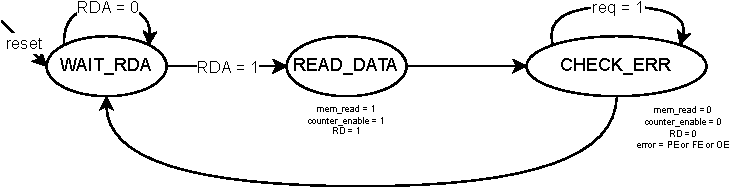
\includegraphics[width=\linewidth]{img/uart_B.pdf}
    \end{minipage}
    \caption{Automi dei sistemi A e B}
    \label{fig:uart}
\end{figure}

\begin{figure}[h]
    \centering
    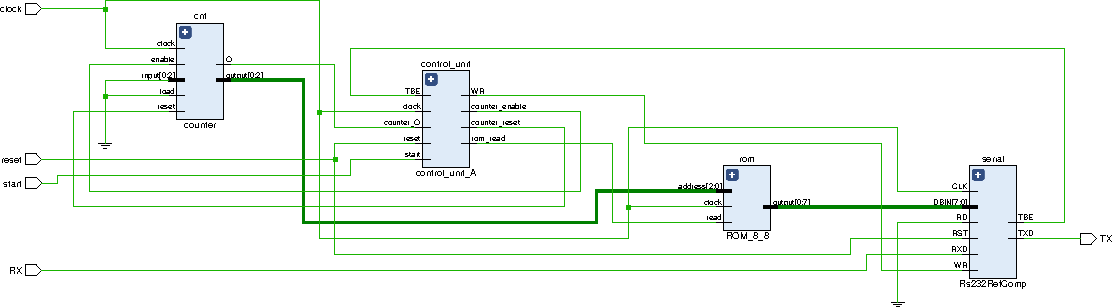
\includegraphics[width=\linewidth]{img/10_UART-RS232_A.pdf}
    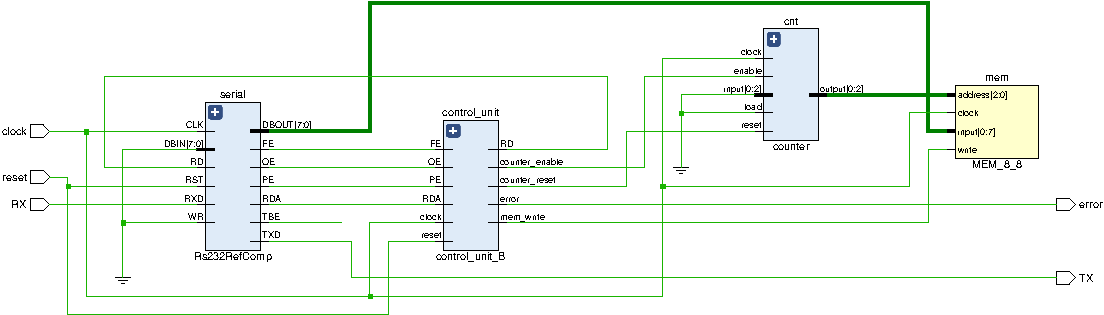
\includegraphics[width=\linewidth]{img/10_UART-RS232_B.pdf}
    \caption{Schema a blocchi del sistema di comunicazione seriale}
    \label{fig:10_UART-RS232}
\end{figure}

\subsubsection{Implementazione}
Si parte dal nodo A:

\begin{code}
    \inputminted{vhdl}{vhdl/uart_system_A.vhd}
    \caption{Implementazione del sistema A}
    \label{cod:uart_system_A}
\end{code}

\begin{code}
    \inputminted{vhdl}{vhdl/uart_control_unit_A.vhd}
    \caption{Implementazione dell'unità di controllo del sistema A}
    \label{cod:uart_control_unit_A}
\end{code}

\paragraph{Funzionamento generale.}
Il nodo A è progettato per inviare dati serialmente attraverso un'interfaccia UART a un altro nodo (B). L'unità A contiene una memoria ROM con 8 locazioni di 1 byte ciascuna e un contatore per scandire le locazioni della ROM. Quando il segnale di scrittura (\texttt{WR}) viene asserito, un byte viene letto dalla ROM e trasmesso tramite UART. Il trasferimento avviene sotto il controllo della \texttt{control\_unit\_A}, che coordina il flusso dei dati e la comunicazione seriale.

I componenti principali del nodo A sono:

\begin{enumerate}
    \item \texttt{ROM\_8\_8}: una memoria ROM che contiene 8 byte. Il contatore determina quale locazione della ROM viene letta.
    \item \texttt{counter}: tiene traccia dell'indirizzo della ROM e permette di scandire sequenzialmente i dati.
    \item \texttt{RS232RefComp} (UART\_A): un'unità UART che gestisce la trasmissione seriale dei dati.
    \item \texttt{control\_unit\_A}: coordina le operazioni di lettura dalla ROM e di scrittura sulla UART.
\end{enumerate}

Il processo di trasmissione avviene in questo modo:

\begin{itemize}
    \item Il segnale di \texttt{start} avvia il trasferimento.
    \item Il contatore inizia a scansionare le locazioni della ROM.
    \item I dati vengono letti dalla ROM e inviati alla UART.
    \item Quando il segnale \texttt{TBE} (Transmitter Buffer Empty) indica che la UART è pronta per trasmettere un nuovo byte, il segnale WR viene attivato per scrivere i dati.
    \item Il processo continua fino a quando tutti gli 8 byte della ROM sono stati inviati.
\end{itemize}

\paragraph{Struttura del codice.}
L'implementazione in VHDL segue un'architettura \texttt{structural} [Codice sorgente \ref{cod:uart_system_A}], con i seguenti componenti interconnessi:

\begin{enumerate}
    \item \texttt{control\_unit\_A} [Codice sorgente \ref{cod:uart_control_unit_A}]: questo modulo governa il processo di trasmissione:
    \begin{itemize}
        \item Asserisce il segnale \texttt{counter\_enable} per far avanzare il contatore.
        \item Attiva il segnale \texttt{rom\_read} per leggere il byte dalla ROM.
        \item Controlla il segnale \texttt{WR} per avviare la trasmissione tramite UART.
        \item Monitora il segnale \texttt{TBE} per evitare di sovrascrivere il buffer della UART prima che sia pronto.
    \end{itemize}
    \item \texttt{ROM\_8\_8} [Codice sorgente \ref{cod:ROM_8_8}]:
    \begin{itemize}
        \item Memorizza 8 byte di dati.
        \item Viene indirizzata dal contatore (\texttt{rom\_address}).
        \item Quando il segnale \texttt{rom\_read} è attivo, la ROM fornisce il valore della locazione corrente in \texttt{DBIN} (Data Bus IN).
    \end{itemize}
    \item \texttt{counter} [Codice sorgente \ref{cod:counter_risingedge}]:
    \begin{itemize}
        \item Tieni traccia dell'indirizzo della ROM.
        \item Avanza quando \texttt{counter\_enable} è attivo.
        \item Si azzera quando \texttt{counter\_reset} è attivato.
        \item Il valore del contatore viene usato come indirizzo della ROM.
    \end{itemize}
    \item \texttt{RS232RefComp} [Codice sorgente \ref{cod:RS232RefComp}]:
    \begin{itemize}
        \item Trasmette i dati serialmente tramite il segnale \texttt{TX}.
        \item Prende i dati da \texttt{DBIN} quando \texttt{WR} è attivo.
        \item Segnala con \texttt{TBE} quando il buffer è pronto per un nuovo byte.
        \item Usa il segnale \texttt{RX} per ricevere dati.
    \end{itemize}
\end{enumerate}

A seguire il nodo B:

\begin{code}
    \inputminted{vhdl}{vhdl/uart_system_B.vhd}
    \caption{Implementazione del sistema B}
    \label{cod:uart_system_B}
\end{code}

\begin{code}
    \inputminted{vhdl}{vhdl/uart_control_unit_B.vhd}
    \caption{Implementazione dell'unità di controllo del sistema B}
    \label{cod:uart_control_unit_B}
\end{code}

\paragraph{Funzionamento generale.}
Il nodo B è progettato per ricevere dati serialmente tramite UART, decodificarli e memorizzarli in una memoria MEM. Funziona in modo speculare al nodo A, ma con una logica inversa:

\begin{itemize}
    \item A trasmette, B riceve.
    \item A legge da ROM, B scrive in MEM.
\end{itemize}

Il flusso dei dati nel nodo B è il seguente:

\begin{enumerate}
    \item Il segnale \texttt{RX} riceve i dati trasmessi dall'unità A tramite UART.
    \item L'unità \texttt{RS232RefComp} (UART\_B) converte il segnale seriale in un byte parallelo e lo pone su \texttt{DBOUT}.
    \item Quando un nuovo dato è disponibile (\texttt{RDA = 1}), l'unità \texttt{RS232RefComp} attiva il segnale \texttt{RD} per leggere il dato dalla UART.
    \item Il contatore avanza per selezionare la prossima locazione della memoria MEM.
    \item Il dato ricevuto viene scritto in MEM alla locazione indicata dal contatore.
    \item Se si verifica un errore di trasmissione (errore di parità, errore di framing o errore di overrun), il segnale \texttt{error} viene asserito.
\end{enumerate}

\paragraph{Struttura del codice.}
L'implementazione in VHDL segue un'architettura \texttt{structural} [Codice sorgente \ref{cod:uart_system_A}], con i seguenti componenti interconnessi:

\begin{enumerate}
    \item \texttt{control\_unit\_B} [Codice sorgente \ref{cod:uart_control_unit_B}]: questo modulo coordina il processo di ricezione e memorizzazione dei dati:
    \begin{itemize}
        \item Attiva il segnale \texttt{RD} per leggere il dato dalla UART quando \texttt{RDA} è alto (dato pronto).
        \item Controlla il segnale \texttt{mem\_write} per scrivere il dato ricevuto nella memoria MEM.
        \item Gestisce il contatore per scandire le locazioni della MEM.
        \item Monitora eventuali errori di trasmissione (\texttt{PE}, \texttt{FE}, \texttt{OE}) e attiva il segnale \texttt{error} in caso di problemi.
    \end{itemize}
    \item \texttt{MEM\_8\_8} [Codice sorgente \ref{cod:MEM_8_8}]: una memoria RAM che salva gli 8 byte ricevuti:
    \begin{itemize}
        \item \texttt{write}: controlla se il dato deve essere scritto.
        \item \texttt{address}: seleziona la locazione di memoria (incrementato dal contatore).
        \item \texttt{input}: riceve il valore da \texttt{DBOUT} (uscita della UART).
    \end{itemize}
    \item \texttt{counter} [Codice sorgente \ref{cod:counter_risingedge}]: tiene traccia della posizione di scrittura nella MEM:
    \begin{itemize}
        \item Avanza quando viene ricevuto un byte e il segnale \texttt{counter\_enable} è attivo.
        \item Si resetta quando il segnale \texttt{counter\_reset} viene attivato.
        \item Il valore attuale del contatore viene usato come indirizzo della MEM.
    \end{itemize}
    \item \texttt{RS232RefComp} [Codice sorgente \ref{cod:RS232RefComp}]: modulo che gestisce la comunicazione seriale:
    \begin{itemize}
        \item \texttt{RXD} riceve il segnale seriale.
        \item \texttt{DBOUT} fornisce il byte ricevuto.
        \item \texttt{RDA} si attiva quando un nuovo byte è pronto.
        \item \texttt{PE}, \texttt{FE}, \texttt{OE} segnalano errori di trasmissione.
    \end{itemize}
\end{enumerate}

\subsubsection{Simulazione}
Per effettuare la simulazione il primo passo da compiere è la stesura del testbench. Prima di discuterne, è stato riportato il seguente codice:

\begin{code}
    \inputminted{vhdl}{vhdl/serial_tb.vhd}
    \caption{Testbench del sistema di comunicazione seriale}
    \label{cod:serial_tb}
\end{code}

Il testbench è progettato per verificare il funzionamento del sistema composto dalle unità A e B, simulando la comunicazione seriale tra di esse. Il test si concentra sulla trasmissione di dati dall’unità A all’unità B attraverso l’interfaccia UART.

La prima operazione svolta è stata la dichiarazione di un’entity. Si può notare che il corpo dell’entity è vuoto, poiché il testbench non rappresenta un componente hardware da implementare, ma serve esclusivamente per la simulazione e la verifica del corretto funzionamento del sistema.

\paragraph{Struttura del testbench.}
Il testbench è strutturato nel seguente modo:

\begin{enumerate}
    \item Dichiarazione dei componenti: il testbench include le due unità principali:
    \begin{itemize}
        \item \texttt{system\_A} (trasmettitore): legge dati dalla ROM e li invia via UART.
        \item \texttt{system\_B} (ricevitore): riceve i dati via UART e li memorizza in MEM.
    \end{itemize}
    \item Segnali e costanti:
    \begin{itemize}
        \item \texttt{CLK\_period = 20 ns}: definisce il periodo del clock.
        \item \texttt{clock}: segnale di clock condiviso tra A e B.
        \item \texttt{reset}: segnale di reset iniziale per azzerare i sistemi.
        \item \texttt{start}: comando per avviare la trasmissione in \texttt{system\_A}.
        \item \texttt{uart\_line}: simula la linea seriale tra TX di A e RX di B.
        \item \texttt{error}: controlla se si verificano errori di ricezione in B.
    \end{itemize}
    \item Processi principali:
    \begin{itemize}
        \item \texttt{CLK\_process}:
        \begin{itemize}
            \item Alterna il segnale clock tra `0' e `1' con un periodo di 20 ns.
            \item Questo simula un clock a 50 MHz che sincronizza entrambi i sistemi.
        \end{itemize}
        \item \texttt{stim\_proc}:
        \begin{itemize}
            \item Attesa di 100 ns: permette al sistema di stabilizzarsi.
            \item Reset disattivato (\texttt{reset <= `0'}): permette l’avvio del sistema.
            \item Start attivato per 20 ns (\texttt{start <= `1'}, poi \texttt{start <= `0'}): inizia la trasmissione dati da A a B.
            \item Attesa indefinita (\texttt{wait}): permette al testbench di eseguire la simulazione fino alla fine del tempo specificato.
        \end{itemize}
    \end{itemize}
    \item Connessioni tra i componenti:
    \begin{itemize}
        \item \texttt{system\_A} trasmette (TX) sulla linea \texttt{uart\_line}.
        \item \texttt{system\_B} riceve (RX) dalla stessa linea \texttt{uart\_line}.
        \item Il testbench non verifica il TX di B, quindi è lasciato scollegato (\texttt{open}).
        \item L'errore di ricezione viene monitorato tramite il segnale \texttt{error}.
    \end{itemize}
\end{enumerate}

\paragraph{Configurazione della seriale.} Il sistema simulato ha un clock di 50 MHz, come richiesto dalla specifica del componente RS232 utilizzato. Per rendere il processo di simulazione non eccessivamente lungo, è stato impostaot un baud rate di 115200. Questo significa che il componente RS232 trasmette 115200 bit al secondo. Il clock dell'unità di trasmissione e quello dell'unità di ricezione, 16 volte più veloce della prima, devono essere impostati adeguatamente:

\begin{align*}
    n_{fronti\_TX} = \frac{50 \cdot 10^6}{115200} = 434 \\
    n_{fronti\_RX} = 434 / 16 = 27
\end{align*}

\begin{figure}[h]
    \centering
    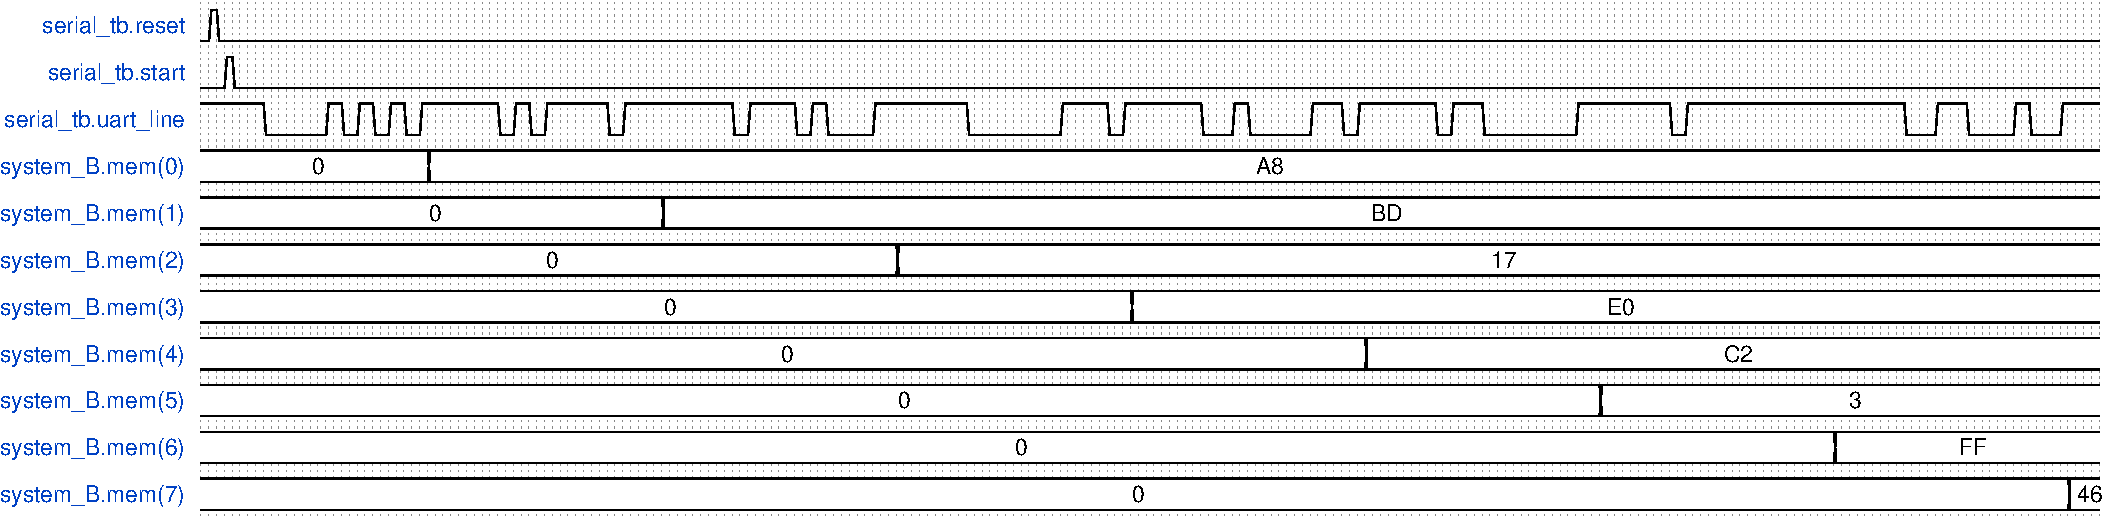
\includegraphics[width=\linewidth]{img/serial_tb.pdf}
    \caption{Simulazione del sistema di comunicazione seriale}
    \label{fig:serial_tb}
\end{figure}
